   %% abtex2-modelo-relatorio-tecnico.tex, v-1.7.1 laurocesar
%% Copyright 2012-2013 by abnTeX2 group at http://abntex2.googlecode.com/ 
%%
%% This work may be distributed and/or modified under the
%% conditions of the LaTeX Project Public License, either version 1.3
%% of this license or (at your option) any later version.
%% The latest version of this license is in
%%   http://www.latex-project.org/lppl.txt
%% and version 1.3 or later is part of all distributions of LaTeX
%% version 2005/12/01 or later.
%%
%% This work has the LPPL maintenance status `maintained'.
%% 
%% The Current Maintainer of this work is the abnTeX2 team, led
%% by Lauro César Araujo. Further information are available on 
%% http://abntex2.googlecode.com/
%%
%% This work consists of the files abntex2-modelo-relatorio-tecnico.tex,
%% abntex2-modelo-include-comandos and abntex2-modelo-references.bib
%%

% ------------------------------------------------------------------------
% ------------------------------------------------------------------------
% abnTeX2: Modelo de Relatório Técnico/Acadêmico em conformidade com 
% ABNT NBR 10719:2011 Informação e documentação - Relatório técnico e/ou
% científico - Apresentação
% ------------------------------------------------------------------------ 
% ------------------------------------------------------------------------

\documentclass[
	% -- opções da classe memoir --
	12pt,				% tamanho da fonte
	openright,			% capítulos começam em pág ímpar (insere página vazia caso preciso)
	oneside,			% para impressão em verso e anverso. Oposto a oneside
	a4paper,			% tamanho do papel. 
	% -- opções da classe abntex2 --
	%chapter=TITLE,		% títulos de capítulos convertidos em letras maiúsculas
	%section=TITLE,		% títulos de seções convertidos em letras maiúsculas
	%subsection=TITLE,	% títulos de subseções convertidos em letras maiúsculas
	%subsubsection=TITLE,% títulos de subsubseções convertidos em letras maiúsculas
	% -- opções do pacote babel --
	english,			% idioma adicional para hifenização
	french,				% idioma adicional para hifenização
	spanish,			% idioma adicional para hifenização
	brazil,				% o último idioma é o principal do documento
	]{abntex2}


% ---
% PACOTES
% ---

% ---
% Pacotes fundamentais 
% ---
\usepackage{cmap}				% Mapear caracteres especiais no PDF
\usepackage{lmodern}			% Usa a fonte Latin Modern
\usepackage[T1]{fontenc}		% Selecao de codigos de fonte.
\usepackage[utf8]{inputenc}		% Codificacao do documento (conversão automática dos acentos)
\usepackage{indentfirst}		% Indenta o primeiro parágrafo de cada seção.
\usepackage{color}				% Controle das cores
\usepackage{graphicx}			% Inclusão de gráficos
\usepackage{subfigure}
% ---

% ---
% Pacotes adicionais, usados no anexo do modelo de folha de identificação
% ---
\usepackage{multicol}
\usepackage{multirow}
% ---
	
% ---
% Pacotes adicionais, usados apenas no âmbito do Modelo Canônico do abnteX2
% ---
\usepackage{lipsum}				% para geração de dummy text
% ---

% ---
% Pacotes de citações
% ---
\usepackage[brazilian,hyperpageref]{backref}	 % Paginas com as citações na bibl
\usepackage[alf]{abntex2cite}	% Citações padrão ABNT

\usepackage{verbatim}
\usepackage{siunitx}%pra usar o ohm
\usepackage{eqnarray,amsmath}
\usepackage[numbered,framed]{matlab-prettifier}

\definecolor{verde}{rgb}{0,0.5,0}
\definecolor{verde_comentario}{rgb}{0.1,0.5,0}
\definecolor{mylilas}{RGB}{170,55,241}

\usepackage{listings}
\lstset{
  style              = Matlab-editor,
  basicstyle         = \mlttfamily,
  escapechar         = ",
  mlshowsectionrules = true,
  literate=%
		{á}{{\'a}}1
		{í}{{\'i}}1
		{é}{{\'e}}1
		{ú}{{\'u}}1
		{ó}{{\'o}}1
		{ô}{{\v{O}}}1
		{â}{{\v{a}}}1
		{ã}{{\~{a}}}1
		{õ}{{\~{o}}}1
		{ç}{{\c{c}}}1
		{Á}{{\'A}}1
		{Í}{{\'I}}1
		{É}{{\'E}}1
		{Ú}{{\'U}}1
		{Ó}{{\'O}}1
		{Ç}{{\c{C}}}1
		{Ô}{{\v{O}}}1
		{Â}{{\v{A}}}1
		{Ã}{{\~{A}}}1
		{Õ}{{\~{O}}}1
}

% --- 
% CONFIGURAÇÕES DE PACOTES
% --- 

% ---
% Configurações do pacote backref
% Usado sem a opção hyperpageref de backref
\renewcommand{\backrefpagesname}{Citado na(s) página(s):~}
% Texto padrão antes do número das páginas
\renewcommand{\backref}{}
% Define os textos da citação
\renewcommand*{\backrefalt}[4]{
	\ifcase #1 %
		Nenhuma citação no texto.%
	\or
		Citado na página #2.%
	\else
		Citado #1 vezes nas páginas #2.%
	\fi}%
% ---

% ---
% Informações de dados para CAPA e FOLHA DE ROSTO
% ---
\titulo{Simulação Hydrone}
\autor{César Bastos da Silva \\
        Dayana\\
        Pedro Miranda Pinheiro \\
        Misaki}
\local{Rio Grande - Brasil}
\data{2020}
\instituicao{%
  Universidade Federal do Rio Grande - FURG
  \par
  Centro de Ciências Computacionais - C3
  \par
  HYDRONE}
\tipotrabalho{Relatório técnico}
% O preambulo deve conter o tipo do trabalho, o objetivo, 
% o nome da instituição e a área de concentração 
\preambulo{Relatório do trabalho .}
% ---

% ---
% Configurações de aparência do PDF final

% alterando o aspecto da cor azul
\definecolor{blue}{RGB}{41,5,195}

% informações do PDF
\makeatletter
\hypersetup{
     	%pagebackref=true,
		pdftitle={\@title}, 
		pdfauthor={\@author},
    	pdfsubject={\imprimirpreambulo},
	    pdfcreator={LaTeX with abnTeX2},
		pdfkeywords={abnt}{latex}{abntex}{abntex2}{relatório técnico}, 
		colorlinks=true,       		% false: boxed links; true: colored links
    	linkcolor=black,          	% color of internal links
    	citecolor=blue,        		% color of links to bibliography
    	filecolor=magenta,      		% color of file links
		urlcolor=blue,
		bookmarksdepth=4
}
\makeatother
% --- 

% --- 
% Espaçamentos entre linhas e parágrafos 
% --- 

% O tamanho do parágrafo é dado por:
\setlength{\parindent}{1.3cm}

% Controle do espaçamento entre um parágrafo e outro:
\setlength{\parskip}{0.2cm}  % tente também \onelineskip

% ---
% compila o indice
% ---
\makeindex
% ---

% ----
% Início do documento
% ----
\begin{document}

% Retira espaço extra obsoleto entre as frases.
\frenchspacing 

% ----------------------------------------------------------
% ELEMENTOS PRÉ-TEXTUAIS
% ----------------------------------------------------------
% \pretextual

% ---
% Capa
% ---
\imprimircapa
% ---

% ---
% Folha de rosto
% (o * indica que haverá a ficha bibliográfica)
% ---
\imprimirfolhaderosto*
% ---

% ---
% Anverso da folha de rosto:
% ---



\begin{comment}
{
\ABNTEXchapterfont

\vspace*{\fill}

Conforme a ABNT NBR 10719:2011, seção 4.2.1.1.1, o anverso da folha de rosto
deve conter:

\begin{alineas}
  \item nome do órgão ou entidade responsável que solicitou ou gerou o
   relatório; 
  \item título do projeto, programa ou plano que o relatório está relacionado;
  \item título do relatório;
  \item subtítulo, se houver, deve ser precedido de dois pontos, evidenciando a
   sua subordinação ao título. O relatório em vários volumes deve ter um título
   geral. Além deste, cada volume pode ter um título específico; 
  \item número do volume, se houver mais de um, deve constar em cada folha de
   rosto a especificação do respectivo volume, em algarismo arábico; 
  \item código de identificação, se houver, recomenda-se que seja formado
   pela sigla da instituição, indicação da categoria do relatório, data,
   indicação do assunto e número sequencial do relatório na série; 
  \item classificação de segurança. Todos os órgãos, privados ou públicos, que
   desenvolvam pesquisa de interesse nacional de conteúdo sigiloso, devem
    informar a classificação adequada, conforme a legislação em vigor; 
  \item nome do autor ou autor-entidade. O título e a qualificação ou a função
   do autor podem ser incluídos, pois servem para indicar sua autoridade no
   assunto. Caso a instituição que solicitou o relatório seja a mesma que o
   gerou, suprime-se o nome da instituição no campo de autoria; 
  \item local (cidade) da instituição responsável e/ou solicitante; NOTA: No
   caso de cidades homônimas, recomenda-se o acréscimo da sigla da unidade da
   federação.
  \item ano de publicação, de acordo com o calendário universal (gregoriano),
  deve ser apresentado em algarismos arábicos.
\end{alineas}

\vspace*{\fill}
}

% ---
% Agradecimentos
% ---
\begin{agradecimentos}
O agradecimento principal é direcionado a Youssef Cherem, autor do
\nameref{formulado-identificacao} (\autopageref{formulado-identificacao}).

Os agradecimentos especiais são direcionados ao Centro de Pesquisa em
Arquitetura da Informação\footnote{\url{http://www.cpai.unb.br/}} da Universidade de
Brasília (CPAI), ao grupo de usuários
\emph{latex-br}\footnote{\url{http://groups.google.com/group/latex-br}} e aos
novos voluntários do grupo
\emph{\abnTeX}\footnote{\url{http://groups.google.com/group/abntex2} e
\url{http://abntex2.googlecode.com/}}~que contribuíram e que ainda
contribuirão para a evolução do abn\TeX.

\end{agradecimentos}
% ---

% ---
% RESUMO
% ---

% resumo na língua vernácula (obrigatório)
\begin{resumo}
 Segundo a \citeonline[3.1-3.2]{NBR6028:2003}, o resumo deve ressaltar o
 objetivo, o método, os resultados e as conclusões do documento. A ordem e a extensão
 destes itens dependem do tipo de resumo (informativo ou indicativo) e do
 tratamento que cada item recebe no documento original. O resumo deve ser
 precedido da referência do documento, com exceção do resumo inserido no
 próprio documento. (\ldots) As palavras-chave devem figurar logo abaixo do
 resumo, antecedidas da expressão Palavras-chave:, separadas entre si por
 ponto e finalizadas também por ponto.

 \vspace{\onelineskip}
    
 \noindent
 \textbf{Palavras-chaves}: latex. abntex. editoração de texto.
\end{resumo}
% ---
\end{comment}
% ---
% inserir lista de ilustrações
% ---
\pdfbookmark[0]{\listfigurename}{lof}
\listoffigures*
\cleardoublepage
% ---

% ---
% inserir lista de tabelas
% ---
%\pdfbookmark[0]{\listtablename}{lot}
%\listoftables*
%\cleardoublepage
% ---

% ---
% inserir lista de abreviaturas e siglas
% ---
\begin{comment}
\begin{siglas}
  \item[Fig.] Area of the $i^{th}$ 
  \item[456] Isto é um número
  \item[123] Isto é outro número
  \item[lauro cesar] este é o meu nome
\end{siglas}
\end{comment}
% ---

% ---
% inserir lista de símbolos
% ---
\begin{comment}
\begin{simbolos}
  \item[$ \Gamma $] Letra grega Gama
  \item[$ \Lambda $] Lambda
  \item[$ \zeta $] Letra grega minúscula zeta
  \item[$ \in $] Pertence
\end{simbolos}
\end{comment}
% ---

% ---
% inserir o sumario
% ---
\pdfbookmark[0]{\contentsname}{toc}
\tableofcontents*
\cleardoublepage
% ---


% ----------------------------------------------------------
% ELEMENTOS TEXTUAIS
% ----------------------------------------------------------
\textual

% ----------------------------------------------------------
%%%%%%%%%%%%%%%%%%%%%%%%%%%%%%%%%%%%%%%%%%%%%%%%%%%%%%%%%%%%%%%%%%%%%%%%%%%%%%%%%%%%%%%%%%%%%%%%%%%%%%%%%%%%%%%%%%%%%%%%%%%%%%%%%%%%%%%%%%%%%%%%    COMEÇA AQUI PARA ESCREVER
%%%%%%%%%%%%%%%%%%%%%%%%%%%%%%%%%%%%%%%%%%%%%%%%%%%%%%%%%%%%%%%%%%%%%%%%%%%%%%%%%%%%%%%%%%%%%%%%%%%%%%%%%%%%%%%%%%%%%%%%%%%%%%%%%%%%%%%%%%%%%%%%%%%%%%%%%%%%%%%%%%%%%%%%%%%%%%%%%%%%%%%%%%%%%%%%%%%%%%%%%%%%%%%%%%%%%%%%
% ----------------------------------------------------------
% \chapter*[Introdução]{Introdução}
% \addcontentsline{toc}{chapter}{Introdução}

\chapter{Dinâmica}
%\begin{lstlisting}[caption={Proposta},label={codigoArmando},firstnumber=181]
%\input{din}
%\end{lstlisting}

%\lstlistoflistings

\section{Função \textit{actuator(this, dwF, dv, dw)}}
Função que calcula atuação nas hélices, tendo como entrada o objeto definido, e algumas variáveis desse objeto: a velocidade $dwF$ (velocidade angular de altitude calculado), velocidade $dv$ (velocidade linear calculado na função \textit{controllerPos(this, ref)}) e velocidade $dw$ (velocidade angular calculado na função \textit{controllerPos(this, ref)}) 

Aqui (código \ref{lst:wh}) é calculado a velocidade de rotação que permite o veículo permanecer em equilíbrio em relação a altitude (hover) (mais na seção \ref{sec:equil}). 


\lstinputlisting[language = Matlab, caption={Parte da função \textit{actuator(this, dwF, dv, dw)}: variável \textit{wh}},label={lst:wh},firstnumber=185,linerange={5-9}]{codigos/din.m}
%firstline=37, lastline=45 ou ,linerange={37-45,48-50}


No trecho a seguir (código \ref{lst:DAr}) define a matriz que indica quais motores serão acionados de acordo com a situação de deslocamento dependendo do condicional, que verifica em qual ambiente que o veículo se encontra. Onde as linhas da matriz indicam os motores (para 0 não aciona, para 1 aciona, e o sinal indica a direção do movimento do veículo), e as colunas os tipos de movimento (em $z$, $xy$, roll, pitch, yaw). 

\lstinputlisting[language = Matlab, caption={Parte da função \textit{actuator(this, dwF, dv, dw)}: variável $D$ para ambiente aéreo}, label={lst:DAr}, firstnumber=191, linerange={11-22}]{codigos/din.m}
%firstline=37, lastline=45 ou ,linerange={37-45,48-50}

No caso do acionamento no ambiente aéreo atribui-se a matriz a seguir (equação \ref{eq:DAr})
\begin{equation}
    D =
    \begin{bmatrix}
        1 & 0 & 0 & -1 & 1 \\
        1 & 0 & 1 & 0 & -1 \\
        1 & 0 & 0 & 1 & 1 \\
        1 & 0 & -1 & 0 & -1 
    \end{bmatrix}
    \label{eq:DAr}
\end{equation}

E no código \ref{lst:DAqua} apresenta a a matriz caso o veículo se encontre no meio aquático.

\lstinputlisting[language = Matlab, caption={Parte da função \textit{actuator(this, dwF, dv, dw)}: variável $D$ para ambiente aquático}, label={lst:DAqua},firstnumber=182,linerange={23-31}]{codigos/din.m}
%firstline=37, lastline=45 ou ,linerange={37-45,48-50}

Enquanto, para o caso do meio subaquático atribui-se a matriz a seguir (equação \ref{eq:DAqua}):

\begin{equation}
    D =
    \begin{bmatrix}
        1 & 0 & 0 & -1 & 0 \\
        1 & 1 & 0 & 0 & -1 \\
        1 & 0 & 0 & 1 & 0 \\
        1 & 1 & 0 & 0 & -1 
    \end{bmatrix}
    \label{eq:DAqua}
\end{equation}

Na variável seguinte (código \ref{lst:w}) é atribuído a $w$ junção de todas as velocidades calculadas ($dv$ e $dw$) junto com as velocidades com ação de controle ($dwF$) e equilíbrio ($wh$) em forma matricial.
\lstinputlisting[language = Matlab, caption={Parte da função \textit{actuator(this, dwF, dv, dw)}: variável $w$},label={lst:w},firstnumber=182,linerange={34-48}]{codigos/din.m}
%firstline=37, lastline=45 ou ,linerange={37-45,48-50}

E então, é atribuído a variável $wdes$ (código \ref{lst:wdes}) a matriz que contém a velocidade desejada para os motores já indicando quais serão acionados de acordo com movimento ($D$)
\lstinputlisting[language = Matlab, caption={Parte da função \textit{actuator(this, dwF, dv, dw)}: variável $wdes$},label={lst:wdes},firstnumber=182,linerange={50-53}]{codigos/din.m}
%firstline=37, lastline=45 ou ,linerange={37-45,48-50}

E em seguida (código \ref{lst:updatemot}), é atualizada o estado dos motores usando a função \textit{update(wdes(i), this.dt, this.env)}, no caso,verifica em qual ambiente o veículo se encontra, e atualiza a velocidade desejada.
\lstinputlisting[language = Matlab, caption={Parte da função \textit{actuator(this, dwF, dv, dw)}: variável $mot$},label={lst:updatemot},firstnumber=182,linerange={55-73}]{codigos/din.m}
%firstline=37, lastline=45 ou ,linerange={37-45,48-50}


\section{Função \textit{wh = equilibrium(this)}}
\label{sec:equil}
Função que calcula a velocidade de rotação dos motores no ponto de equilíbrio (tipo hover)

No trecho \ref{lst:phithe} é atribuído as orientações atuais do veículo (ângulo $\phi$ e $\theta$) para verificar e corrigir se necessário para manter o veículo próximo da orientação nula nos ângulos $phi$ e $theta$.
\lstinputlisting[language = Matlab, caption={Parte da função \textit{wh = equilibrium(this)}: variáveis $\phi$ e $\theta$ },label={lst:phithe},firstnumber=182,linerange={79-80}]{codigos/din.m}
%firstline=37, lastline=45 ou ,linerange={37-45,48-50}

Em seguida (código \ref{lst:alpha}) é verificada em qual ambiente o veículo se encontra para determinar o efeito de inclinação desses ângulos.
\lstinputlisting[language = Matlab, caption={Parte da função \textit{wh = equilibrium(this)}: variável $\alpha$},label={lst:alpha},firstnumber=182,linerange={82-95}]{codigos/din.m}
%firstline=37, lastline=45 ou ,linerange={37-45,48-50}

É definido o termo do efeito da força da gravidade (código \ref{lst:grav}) de acordo com o ambiente. Sendo $\rho$ densidade do ambiente, $Vol$ o volume do veículo, $m$ a massa e $g$ a aceleração da gravidade.
\begin{equation}
    g_{term} = |m - \rho Vol| g
\end{equation}
\lstinputlisting[language = Matlab, caption={Parte da função \textit{wh = equilibrium(this)}: variável $grav_{term}$},label={lst:grav},firstnumber=182,linerange={97-101}]{codigos/din.m}
%firstline=37, lastline=45 ou ,linerange={37-45,48-50}

Então é definido o ganho do motor calculado na função \textit{getKf(this)} que se encontra em outro arquivo (ver seção \ref{sec:prop}), onde pode ser calculado ou levantadas por ensaios.
\lstinputlisting[language = Matlab, caption={Parte da função \textit{wh = equilibrium(this)}: variável $k_f$},label={lst:kf},firstnumber=182,linerange={103-119}]{codigos/din.m}
%firstline=37, lastline=45 ou ,linerange={37-45,48-50}

Com todas as variáveis definidas é calculado a variável $wh$ de acordo com o ambiente.
\lstinputlisting[language = Matlab, caption={Parte da função \textit{wh = equilibrium(this)}: variável },label={lst:wh},firstnumber=182,linerange={121-133}]{codigos/din.m}
%firstline=37, lastline=45 ou ,linerange={37-45,48-50}

\section{Função  [at, aa] = getAccel(this, v, q, r)}
\label{sec:getAccel}
Nesta função é calculado a aceleração translacional($at$) e rotacional ($aa$) do veículo, tendo como entrada o objeto, a velocidade linear ($v$) e angular ($q$) medido, e a orientação ($r$) do veículo. 

Inicialmente é determinado a densidade do ambiente ($\rho$) pela função \textit{getRho(this)} que se encontra em outro no arquivo $.m$ (ver seção \ref{sec:prop}).
\lstinputlisting[language = Matlab, caption={Parte da função \textit{getAccel(this, v, q, r)}: variável $\rho$ }, label={lst:rho},firstnumber=182,linerange={139-149}]{codigos/din.m}
%firstline=37, lastline=45 ou ,linerange={37-45,48-50}

Para o cálculo dessa dinâmica é preciso determinar a massa adicional e inércia adicional (código \ref{lst:adicional}), apesar de no meio aéreo seja mínimo. (é considerado a cápsula do veículo na forma esférica), sendo o volume da esfera:
\begin{equation}
    Vol = \frac{4}{3} \pi R^3
\end{equation}
 onde $R$ é o raio da esfera ($rc$).

\lstinputlisting[language = Matlab, caption={Parte da função \textit{getAccel(this, v, q, r)}: variáveis $adde_{mass}$ e $added_{inertia}$ }, label={lst:adicional},firstnumber=182,linerange={151-154}]{codigos/din.m}
%firstline=37, lastline=45 ou ,linerange={37-45,48-50}

\lstinputlisting[language = Matlab, caption={Parte da função \textit{getAccel(this, v, q, r)}: variável $f_1$ }, label={lst:f1},firstnumber=182,linerange={156-162}]{codigos/din.m}
%firstline=37, lastline=45 ou ,linerange={37-45,48-50}

\lstinputlisting[language = Matlab, caption={Parte da função \textit{getAccel(this, v, q, r)}: variável $f_2$ }, label={lst:f2},firstnumber=182,linerange={164-166}]{codigos/din.m}
%firstline=37, lastline=45 ou ,linerange={37-45,48-50}

\lstinputlisting[language = Matlab, caption={Parte da função \textit{getAccel(this, v, q, r)}: variável $f_3$ }, label={lst:f3},firstnumber=182,linerange={168-170}]{codigos/din.m}
%firstline=37, lastline=45 ou ,linerange={37-45,48-50}

\lstinputlisting[language = Matlab, caption={Parte da função \textit{getAccel(this, v, q, r)}: variável $f_4$}, label={lst:f4},firstnumber=182,linerange={172-174}]{codigos/din.m}
%firstline=37, lastline=45 ou ,linerange={37-45,48-50}

\lstinputlisting[language = Matlab, caption={Parte da função \textit{getAccel(this, v, q, r)}: variável $f_5$ }, label={lst:f5},firstnumber=182,linerange={176-178}]{codigos/din.m}
%firstline=37, lastline=45 ou ,linerange={37-45,48-50}


\lstinputlisting[language = Matlab, caption={Parte da função \textit{getAccel(this, v, q, r)}: variável $a_t$}, label={lst:at},firstnumber=182,linerange={180-182}]{codigos/din.m}
%firstline=37, lastline=45 ou ,linerange={37-45,48-50}


\lstinputlisting[language = Matlab, caption={Parte da função \textit{getAccel(this, v, q, r)}: variáveis $peso$ e $empuxo$}, label={lst:pesoempuxo},firstnumber=182,linerange={184-189}]{codigos/din.m}
%firstline=37, lastline=45 ou ,linerange={37-45,48-50}


\lstinputlisting[language = Matlab, caption={Parte da função \textit{getAccel(this, v, q, r)}: variável $dist$}, label={lst:dist},firstnumber=182,linerange={191-192}]{codigos/din.m}
%firstline=37, lastline=45 ou ,linerange={37-45,48-50}

\lstinputlisting[language = Matlab, caption={Parte da função \textit{getAccel(this, v, q, r)}: variável $m_1$ }, label={lst:m1},firstnumber=182,linerange={194-207}]{codigos/din.m}
%firstline=37, lastline=45 ou ,linerange={37-45,48-50}

\lstinputlisting[language = Matlab, caption={Parte da função \textit{getAccel(this, v, q, r)}: variável $m_2$ }, label={lst:m2},firstnumber=182,linerange={209-211}]{codigos/din.m}
%firstline=37, lastline=45 ou ,linerange={37-45,48-50}

\lstinputlisting[language = Matlab, caption={Parte da função \textit{getAccel(this, v, q, r)}: variável $m_3$ }, label={lst:m3},firstnumber=182,linerange={213-215}]{codigos/din.m}
%firstline=37, lastline=45 ou ,linerange={37-45,48-50}

\lstinputlisting[language = Matlab, caption={Parte da função \textit{getAccel(this, v, q, r)}: variável $m_4$ }, label={lst:m4},firstnumber=182,linerange={217-222}]{codigos/din.m}
%firstline=37, lastline=45 ou ,linerange={37-45,48-50}

\lstinputlisting[language = Matlab, caption={Parte da função \textit{getAccel(this, v, q, r)}: variável $a_a$ }, label={lst:aa},firstnumber=182,linerange={224-228}]{codigos/din.m}
%firstline=37, lastline=45 ou ,linerange={37-45,48-50}
\iffalse
\section{Função \textit{dynamics(this)}}


\lstinputlisting[language = Matlab, caption={Parte da função \textit{dynamics(this)}: variáveis $F$ e $M$}, label={lst:FM},firstnumber=182,linerange={233-237}]{codigos/din.m}
%firstline=37, lastline=45 ou ,linerange={37-45,48-50}



\lstinputlisting[language = Matlab, caption={Parte da função \textit{dynamics(this)}: variáveis $F$ e $M$}, label={lst:FM},firstnumber=182,linerange={233-237}]{codigos/din.m}
%firstline=37, lastline=45 ou ,linerange={37-45,48-50}

\lstinputlisting[language = Matlab, caption={Parte da função \textit{dynamics(this)}: variáveis $F$ e $M$}, label={lst:FM},firstnumber=182,linerange={233-237}]{codigos/din.m}
%firstline=37, lastline=45 ou ,linerange={37-45,48-50}

\lstinputlisting[language = Matlab, caption={Parte da função \textit{dynamics(this)}: variáveis $F$ e $M$}, label={lst:FM},firstnumber=182,linerange={233-237}]{codigos/din.m}
%firstline=37, lastline=45 ou ,linerange={37-45,48-50}

\lstinputlisting[language = Matlab, caption={Parte da função \textit{dynamics(this)}: variáveis $F$ e $M$}, label={lst:FM},firstnumber=182,linerange={233-237}]{codigos/din.m}
%firstline=37, lastline=45 ou ,linerange={37-45,48-50}

\lstinputlisting[language = Matlab, caption={Parte da função \textit{dynamics(this)}: variáveis $F$ e $M$}, label={lst:FM},firstnumber=182,linerange={233-237}]{codigos/din.m}
%firstline=37, lastline=45 ou ,linerange={37-45,48-50}

\lstinputlisting[language = Matlab, caption={Parte da função \textit{dynamics(this)}: variáveis $F$ e $M$}, label={lst:FM},firstnumber=182,linerange={233-237}]{codigos/din.m}
%firstline=37, lastline=45 ou ,linerange={37-45,48-50}

\lstinputlisting[language = Matlab, caption={Parte da função \textit{dynamics(this)}: variáveis $F$ e $M$}, label={lst:FM},firstnumber=182,linerange={233-237}]{codigos/din.m}
%firstline=37, lastline=45 ou ,linerange={37-45,48-50}

\fi



\pagebreak

\chapter{Parâmetros do veiculo}
Aqui são declaras os parâmetros do veiculo que serão usadas ao longo da simulação, de acordo com o dado de interesse a ser simulado, como por exemplo, o momento de inercia pode ser de interesse quando se simula algo relacionado a rotação e o coeficiente de arrasto é usado na equação do arrasto, onde um coeficiente de arraste mais baixo indica que o objeto terá menos arraste aerodinâmico ou hidrodinâmico.
%\section*{Massa}
%A massa está relacionada com inercia do corpo, além da eficiência energética.
\lstinputlisting[language = Matlab, caption={Parametros do veiculo},label={parametros do veiculo},firstnumber=2,linerange={2-57}]{codigos/ParamVeic.m}

%\section*{Momentos de inércia}
%Influência na rotação do corpo.
%\lstinputlisting[language = Matlab, caption={Momento de Inércia},label={Momento de inercia},firstnumber=3,linerange={3-7}]{codigos/ParamVeic.m}

%???
%\lstinputlisting[language = Matlab, caption={Parte do código quadhibrido.m},label={Outras propriedades},firstnumber=8,linerange={8-12}]{codigos/ParamVeic.m}

%\section*{Coeficientes de arrasto}
%O coeficiente de arrasto permite quantificar a força de resistência ao ar ou outro fluido por parte de uma dada superfície. É usado na equação do arrasto, onde um coeficiente de arraste mais baixo indica que o objeto terá menos arraste aerodinâmico ou hidrodinâmico. 
%\lstinputlisting[language = Matlab, caption={Coeficientes de arrasto},label={Coeficientes de Arrasto },firstnumber=13,linerange={13-14}]{codigos/ParamVeic.m}


%\section*{Saturação dos ângulos}
%Utilizado para  evitar a singularidade na matriz de rotação.
%\lstinputlisting[language = Matlab, caption={Parte do código quadhibridoproposta.m},label={Saturação de Ângulos},firstnumber=17,linerange={17-22}]{codigos/ParamVeic.m}


%\section*{Motores}
%\lstinputlisting[language = Matlab, caption={Parte do código quadhibridoproposta.m},label={Motor},firstnumber=23,linerange={23-26}]{codigos/ParamVeic.m}

%\section*{Controladores}
%\lstinputlisting[language = Matlab, caption={Parte do código quadhibridoproposta.m},label={Controladores},firstnumber=28,linerange={28-30}]{codigos/ParamVeic.m}


%\lstinputlisting[language = Matlab, caption={Parte do código quadhibridoproposta.m},label={talvez plot},firstnumber=30,linerange={30-32}]{codigos/ParamVeic.m}

%\section*{Parâmetros de ambiente}
%\lstinputlisting[language = Matlab, caption={Parte do código quadhibridoproposta.m},label={Paramentos Ambiente},firstnumber=35,linerange={35-43}]{codigos/ParamVeic.m}


%\lstinputlisting[language = Matlab, caption={Parte do código quadhibridoproposta.m},label={Times},firstnumber=43,linerange={43-57}]{codigos/ParamVeic.m}

\chapter{Parâmetros de hélices e motores}
\label{sec:prop}
Todos os arquivos do simulador que iniciam com o prefixo \emph{prop} estão relacionados à descrição de um conjunto motor-hélice (atuadores do veículo). Sua estrutura principal pode ser verificada na figura \ref{fig:uml-01}.

\begin{figure}[!htb]
    \centering
    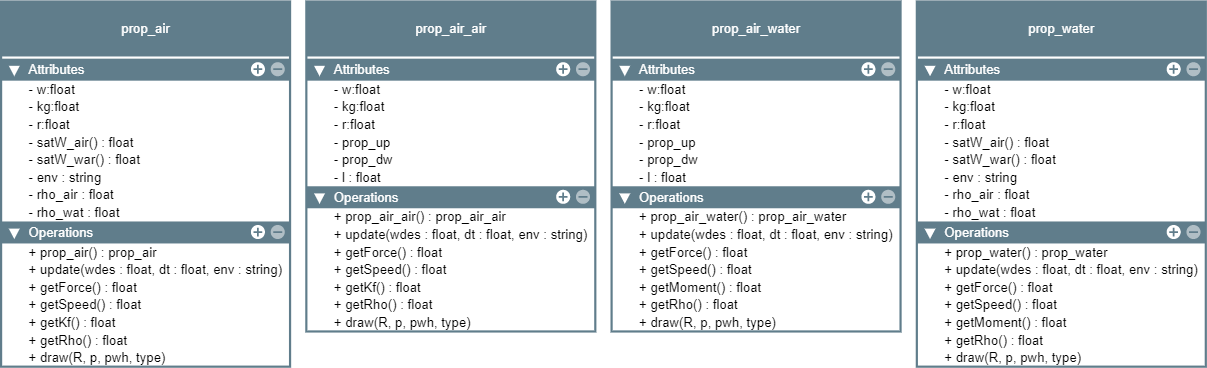
\includegraphics[width=\linewidth]{imagens/uml1.png}
    \caption{Diagrama UML das classes \emph{prop-}.}
    \label{fig:uml-01}
\end{figure}

\section{Classes \emph{prop\_air} e \emph{prop\_water}}
% utilizar \_ para evitar erros
As classes \emph{prop\_air} e \emph{prop\_water} são responsáveis por descrever dois tipos de conjuntos motor-hélice, respectivamente, aéreos e aquáticos. Estas são instanciadas nas classes \emph{prop\_air\_air} e \emph{prop\_air\_water}, nos objetos \emph{prop\_up} e \emph{prop\_dw}, os quais guardam a informação de qual tipo de conjunto é utilizado no ar e na água, respectivamente. Tal estrutura se deve à comparação de desempenho entre conjuntos aéreos e aquáticos para movimentação subaquática.

Conforme pode-se observar no trecho a seguir, a classe \emph{prop\_air}, bem como a classe \emph{prop\_water}, inicia com a declaração de algumas propriedades. Tais propriedades referem-se tanto a parâmetros específicos do conjunto motor-hélice, como, também, a propriedades relacionadas ao meio em que podem estar.

\lstinputlisting[language = Matlab, caption={propriedades da classe prop\_air},label={prop-air-1},firstnumber=3,linerange={3-17}]{codigos/prop_air.m}

Após a definição das propriedades das classes \emph{prop\_air} e \emph{prop\_water}, são criados os métodos das mesmas, os quais são responsáveis pela construção dos objetos, atualização das variáveis simuladas, retorno de valores para o código principal e pelo desenho das hélices na representação gráfica da simulação. O trecho a seguir mostra os métodos da classe \emph{prop\_air}.

\lstinputlisting[language = Matlab, caption={métodos da classe prop\_air},label={prop-air-1},firstnumber=19,linerange={19-91}]{codigos/prop_air.m}


\section{Classes \emph{prop\_air\_air} e \emph{prop\_air\_water}}
Os códigos para as classes \emph{prop\_air\_air} e \emph{prop\_air\_water} são similares entre si, diferindo apenas pela construção dos objetos. Para o primeiro, o atributo \emph{prop\_dw} recebe um objeto da classe \emph{prop\_air}, e para o segundo, o mesmo atributo recebe um objeto da classe \emph{prop\_water}.

Como esperado, as classes \emph{prop\_air\_air} e \emph{prop\_air\_water}, simplesmente agrupam os pares de atuadores, guardando as informações sobre cada um dos conjuntos motor-hélice. Assim, este código chama os métodos para os respectivos tipos de atuadores, conforme necessário.
\chapter{Controlador}

A arquitetura de controle mais utilizada em quadricópteros, possui várias malhas de controles em sua grande maioria em cascata. Onde primeiramente é realizado um controle em relação a posição do veículo e por conseguinte sua orientação. Como a configuração do sentido das hélices do veículo na água é diferente em relação ao ar, diferentes métodos de controle aplicado.

Na Figura \ref{fig:malhacontrole-01} é possível ver a representação gráfica do que está sendo realizado no simulador, onde é possível foram criadas duas grandes malhas correspondentes para cada meio. A explicação da imagem será dada junto ao código, para mostrar como o controle ocorre.

\section{Controle de Posição}

No trecho de código \ref{controle1} é realizado a inicialização do controlador de posição, onde essencialmente são coletados as posições (x, y e z) e o \textit{yaw} de referência, logo após os valores atuais de posição, \textit{yaw} e velocidade x e y são também adquiridos. O controle em z é feito separadamente, então é calculado o erro da posição em x e em y para ser passado para o controlador.


\lstinputlisting[language = Matlab, caption={Aquisição dos valores para realizar o controle de posição},label={controle1},firstnumber=1,linerange={1-15}]{codigos/controlador.m}

\begin{figure}[!htb]
    \centering
    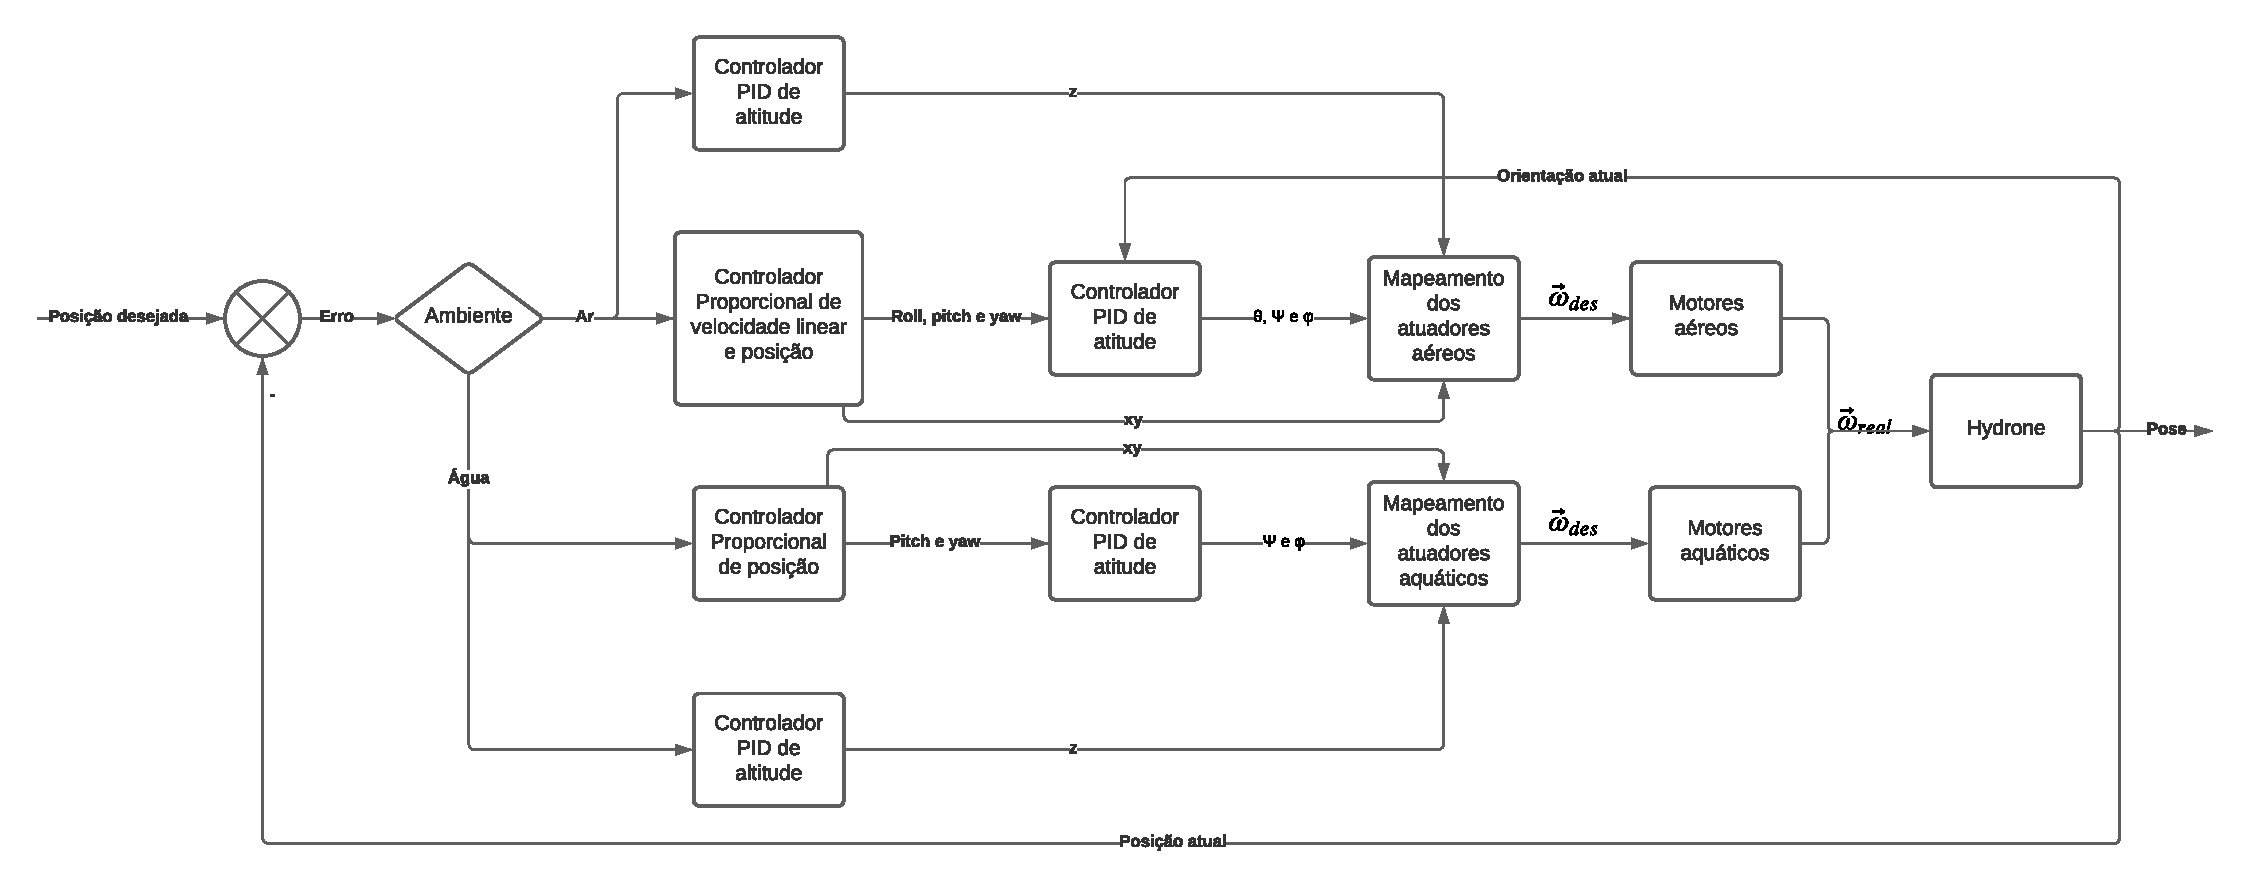
\includegraphics[width=1.4\linewidth, angle =90]{imagens/Controle simulação.pdf}
    \caption{Arquitetura de controle implementada.}
    \label{fig:malhacontrole-01}
\end{figure}

\pagebreak

Seguindo então o diagrama apresentado na Figura \ref{fig:malhacontrole-01} é realizada a verificação do tipo de ambiente, o trecho \ref{controle2} apresenta o controle de posição no ar, onde Kp e Kd são ganhos proporcionais aos erros de posição e velocidade, respectivamente. A variável "R" corresponde a matriz de rotação no eixo z, para mudar os valores de posição e velocidade do referencial local, do veículo, para o global. Por fim, a lei de controle utilizada é apresentada na Equação \ref{controlepos}, sendo ".*", multiplicação de elemento a elemento, gerando valor de referência de \textit{roll} e \textit{pitch} para o ar. Como o controle de x e y no ar é relacionado com a orientação do veículo, o valor de "dv" é zerado.

\lstinputlisting[language = Matlab, caption={Controle de posição no ar},label={controle2},firstnumber=18,linerange={18-36}]{codigos/controlador.m}

\begin{equation}
    \label{controlepos}
    Ang_{ref} =  K_p\begin{bmatrix}
    -1\\
    1
    \end{bmatrix}.*d_p + K_d\begin{bmatrix}
    -1\\
    1
    \end{bmatrix}.*dv
\end{equation}

Caso, o veículo esteja na água, o trecho \ref{controle3} que será utilizado. Na água o controle no plano XY pode ser bastante similar a um veículo diferencial. Primeiramente é calculada a distância euclidiana entre a posição atual e a referência, caso essa distância por maior que um valor de \textit{threshhold} previamente estabelecida o controle será aplicado. Então é coletado e calculado o ângulo entre o alvo e o veículo, tendo seu valor normalizado entre $\pi$ e $-\pi$. Diferentemente do controle no ar, na águam é aplicada uma lei de controle relacionada ao ângulo e a distância até o alvo, podendo ser observado na Equação \ref{equacaoposagua}.

\lstinputlisting[language = Matlab, caption={Controle de posição na água},label={controle3},firstnumber=38,linerange={38-77}]{codigos/controlador.m}

\begin{equation}
    \label{equacaoposagua}
    d_v = k_vd + k_a|\alpha|^2
\end{equation}

\section{Controle de Altitude}

Conforme pode ser visto na Figura \ref{fig:malhacontrole-01} paralelo ao controle de posição é realizado o controle de altitude, o qual está apresentado no trecho \ref{controle4}, onde é utilizada a função "\textit{getU}" que será explicada na Seção \ref{pid}, onde sua grande diferença entre a água e o ar, são os ganhos distintos, determinados no construtor da classe.


\lstinputlisting[language = Matlab, caption={Controle de altitude no ar e na água },label={controle4},firstnumber=80,linerange={80-84}]{codigos/controlador.m}

\section{Controle de Atitude}

Na Figura \ref{fig:malhacontrole-01} após a execução do controlador de posição é realizado o controle de atitude, visto que os valores de referência a serem utilizados é a ação de controle do controlador de posição. No ar, basicamente é aplicado um PID utilizando a "\textit{getU}", podendo ser visto no trecho \ref{controle5}, resultando em 3 sinais de controle, para a correção dos ângulos $\theta$, $\phi$ e $\psi$.

\lstinputlisting[language = Matlab, caption={Controle de atitude no ar},label={controle5},firstnumber=88,linerange={88-100}]{codigos/controlador.m}

Como o Hydrone é subatuado na água, ele não consegue controlar diretamente o $\theta$ do veículo,  conforme é apresentado no trecho \ref{controle6}. Realizando um PID tanto para os ângulos $\phi$ e $\psi$.

\lstinputlisting[language = Matlab, caption={Controle de atitude na água},label={controle6},firstnumber=101,linerange={101-113}]{codigos/controlador.m}

Após todos controles implementados, as contribuições correspondentes ao movimento vertical, longitudinal e de orientação do veículos são manipulador a função "\textit{actuator}", previamente apresentada, resultado nas velocidades desejadas a serem aplicadas nos motores.

\section{Função \textit{getU}(this, rn, yn, dt)}\label{pid}

A função \textit{getU} é a base dos controladores PID's que são utilizados ao longo da simulação, uma explicação sobre alguns detalhes sobre sua implementação são bastante importantes.

Presente como uma função da classe "pid", essa função consiste basicamente em aplicar a lei de controle estabelecida. Inicialmente, conforme pode ser visto no trech \ref{pid1}, são apresentadas três constantes, onde $\gamma$ e $\beta$ são variáveis que ajustam o ganho diretamente, enquanto $\alpha$ corresponde a determinação do tempo do filtro aplicado no cálculo do erro derivativo.


\lstinputlisting[language = Matlab, caption={Parâmetros padrões do algoritmo de controle},label={pid1},firstnumber=50,linerange={50-53}]{codigos/pid.m}

No trecho \ref{pid2} é apresentado o cálculo do erro derivativo, o qual, além do cálculo normal do erro é adicionado um filtro passa-baixa, a fim de eliminar possível valores alta frequência gerados na variação do erro. O valor de $\alpha$ é $0,1$ correspondendo ao tempo de corte do filtro ser $10\%$ do tempo do tempo derivativo.

\lstinputlisting[language = Matlab, caption={Cálculo do erro derivativo com aplicação de um filtro passa-baixa.},label={pid2},firstnumber=64,linerange={64-75}]{codigos/pid.m}

Por fim, como o sistema é todo discretizado, existem diferentes maneiras de se discretizar o PID, no caso, o utilizado foi o modelo do PID ótimo, conforme visto no trecho \ref{pid3}.

\lstinputlisting[language = Matlab, caption={PID ótimo implementado},label={pid3},firstnumber=76,linerange={76-89}]{codigos/pid.m}

\addcontentsline{toc}{chapter}{Conclusão}


% ----------------------------------------------------------
% ELEMENTOS PÓS-TEXTUAIS
% ----------------------------------------------------------
\postextual

% ----------------------------------------------------------
% Referências bibliográficas
% ----------------------------------------------------------
\bibliography{abntex2-modelo-references}
\end{document}
